\FloatBarrier
\begin{figure}[!h]
\centering
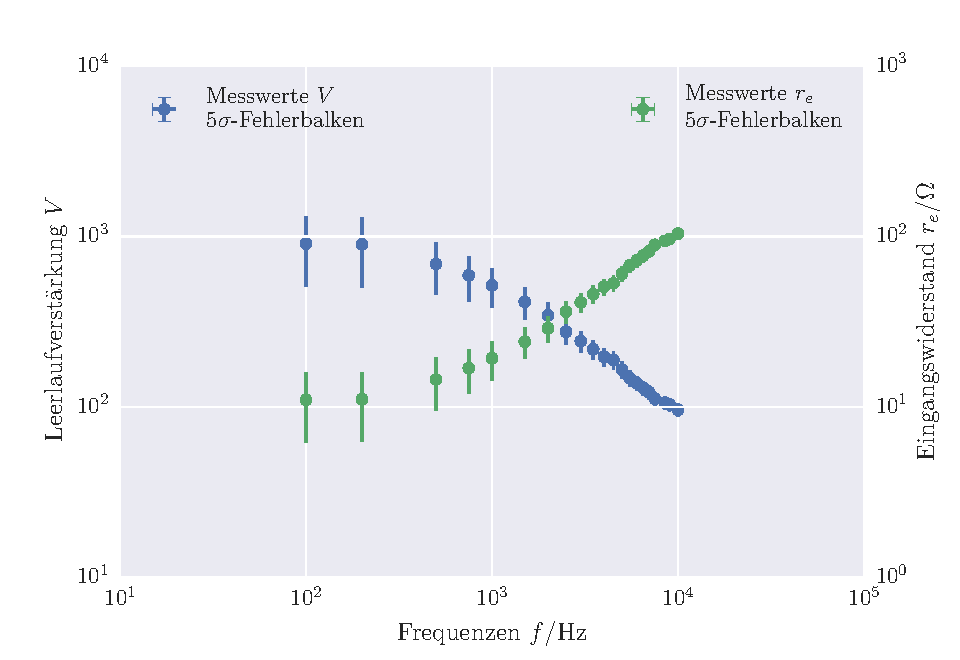
\includegraphics[scale=1]{../Grafiken/Amperemeter_Leerlaufverstaerkung_Eingangswiderstand.pdf}
\caption{Doppellogarithmische Darstellung des Leerlaufverstärkung $V$ (linke Skala, blaue) und des
	Eingangswiderstandes $r_{\mathrm{e}}$
	(rechte Skala, grün) der Amperemeterschaltung in Abhängigkeit der
	Frequenz.\label{fig:amperemeter_leerlaufverstaerkung_eingangswiderstand}}
\end{figure}
\FloatBarrier